\section{Results}
\label{sec:results}

\subsection{Self-Critique Produces Large, Consistent Improvement}
\label{sec:main_results}

\tabref{tab:main} presents the main results.
All \selfrefine conditions significantly outperform the baseline, with win rates of 80--87\% and very large effect sizes ($d > 1.5$).
A single \critiquerevise iteration achieves an 80\% win rate ($p < 0.001$, Cohen's $d = 2.02$), establishing self-critique as a highly effective strategy for improving story quality.

\begin{table}[t]
\centering
\caption{Main results: pairwise comparison of each condition against the \baseline. Win\% indicates how often the condition was preferred over baseline by the blind judge. Mean $\Delta$ is the average score difference across six dimensions. All $p$-values from Wilcoxon signed-rank tests with Bonferroni correction.}
\label{tab:main}
\resizebox{\textwidth}{!}{
\begin{tabular}{@{}lcccccc@{}}
\toprule
\textbf{Condition} & \textbf{Win\%} & \textbf{Tie\%} & \textbf{Loss\%} & \textbf{Mean $\Delta$} & \textbf{$p$-value} & \textbf{Cohen's $d$} \\
\midrule
\selfrefine $\times$1 & {\bf 80} & 7 & 13 & {\bf +0.66} & $< 0.001$ & {\bf 2.02} \\
\selfrefine $\times$2 & {\bf 87} & 7 & 7 & +0.64 & $< 0.001$ & 1.85 \\
\selfrefine $\times$3 & 80 & 7 & 13 & +0.60 & $< 0.001$ & 1.70 \\
\bestofn ($N\!=\!4$) & 60 & 0 & 40 & +0.02 & 0.798 & 0.04 \\
\bestofn + Refine & {\bf 87} & 7 & 7 & +0.54 & $< 0.001$ & 1.52 \\
\bottomrule
\end{tabular}
}
\end{table}

The \bestofn condition without refinement is the outlier: its 60\% win rate is not statistically significant ($p = 0.80$, $d = 0.04$), indicating that self-selection without structured critique is largely ineffective.
Adding one refinement pass to \bestofn recovers strong performance (87\% win rate), confirming that critique---not generation diversity---drives improvement.

\subsection{Diminishing Returns After the First Iteration}
\label{sec:trajectory}

\begin{figure}[t]
\centering
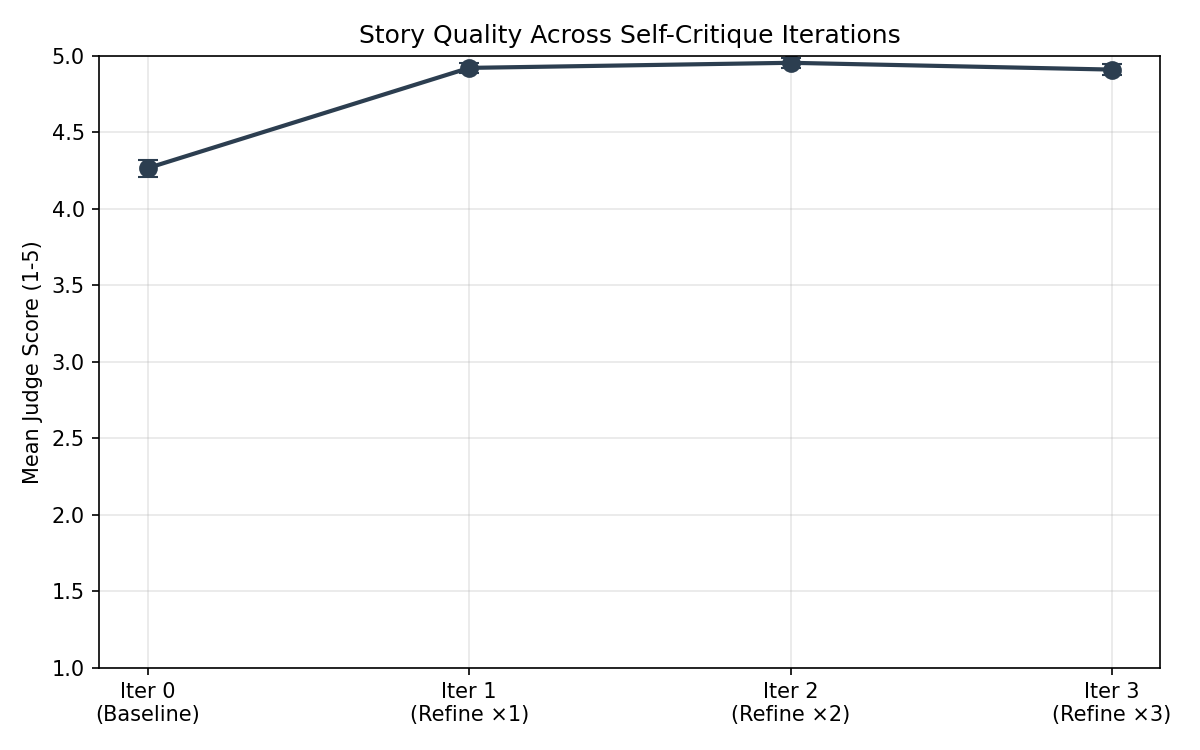
\includegraphics[width=0.7\linewidth]{figures/iteration_trajectory.png}
\caption{Mean score across six evaluation dimensions as a function of \critiquerevise iterations. The first iteration produces a large jump from the baseline (~4.25 to ~4.93); subsequent iterations plateau and show signs of regression by iteration~3.}
\label{fig:trajectory}
\end{figure}

\Figref{fig:trajectory} shows the trajectory of mean scores across iterations.
The pattern is clear: iteration 0 to 1 produces a large jump (baseline $\sim$4.25 $\rightarrow$ refined $\sim$4.93), iteration 1 to 2 adds marginal gain ($\sim$4.96), and iteration 2 to 3 slightly declines ($\sim$4.91).
The first critique captures the most actionable feedback; subsequent iterations have less material to improve and may introduce overcorrection.

\subsection{Improvement Is Strongest in Creative Dimensions}
\label{sec:dimensions}

\begin{figure}[t]
\centering
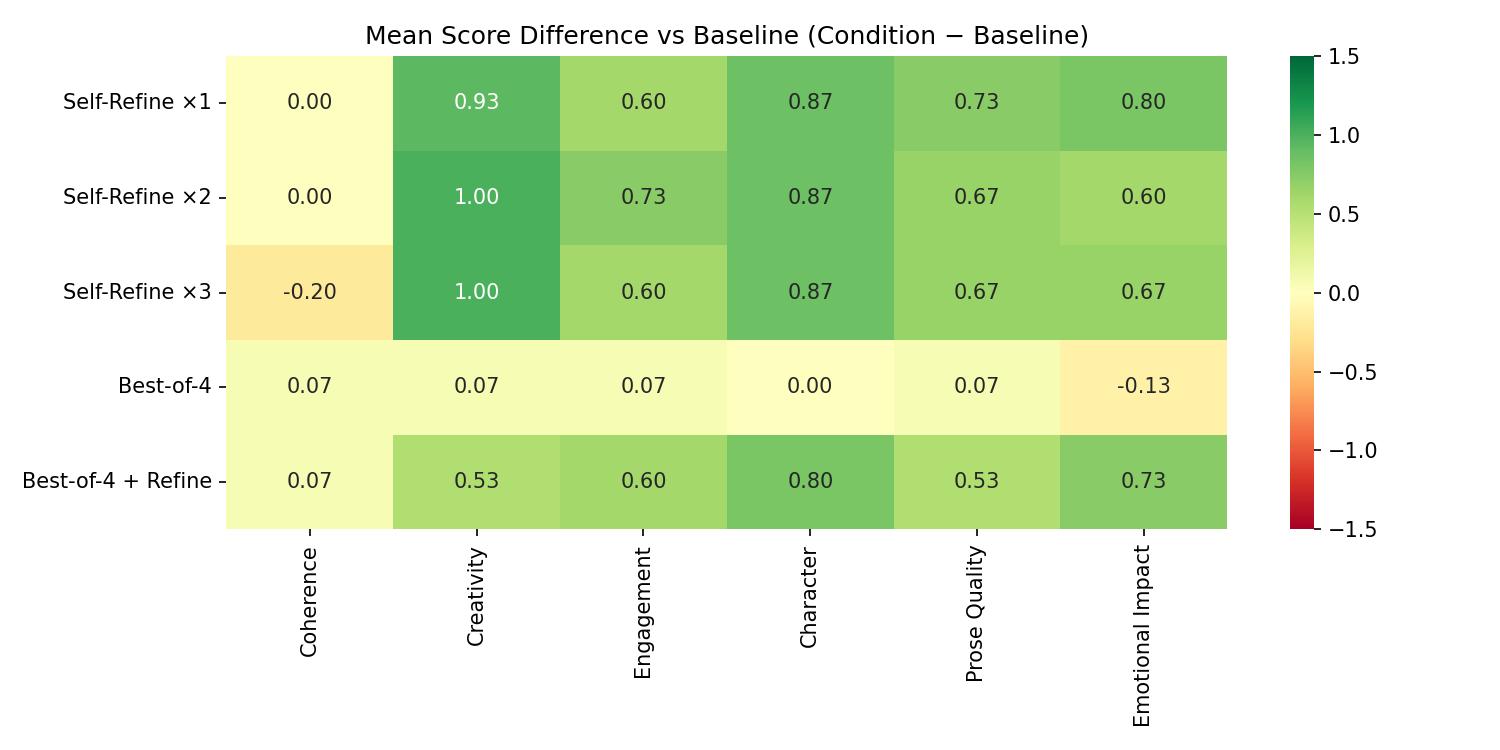
\includegraphics[width=0.75\linewidth]{figures/score_diffs_heatmap.png}
\caption{Score differences (condition $-$ baseline) per evaluation dimension. Creativity and character development show the largest, most consistent gains. Coherence starts high and slightly declines at iteration~3.}
\label{fig:heatmap}
\end{figure}

\Figref{fig:heatmap} and \tabref{tab:dimensions} reveal where self-critique helps most.
Creativity and character development show the largest gains (+0.87 to +1.00 points), consistent across all \selfrefine iterations.
Prose quality and emotional impact show moderate improvement (+0.60 to +0.80).
Coherence, by contrast, starts at or near ceiling and shows no improvement at iteration 1---and actually \emph{declines} at iteration 3 ($-0.20$), suggesting that excessive revision can introduce plot inconsistencies.

\begin{table}[t]
\centering
\caption{Per-dimension score differences (condition $-$ baseline) for \selfrefine iterations. Best values per dimension in \textbf{bold}.}
\label{tab:dimensions}
\begin{tabular}{@{}lccc@{}}
\toprule
\textbf{Dimension} & $\times$\textbf{1} & $\times$\textbf{2} & $\times$\textbf{3} \\
\midrule
Creativity & +0.93 & {\bf +1.00} & {\bf +1.00} \\
Character & {\bf +0.87} & {\bf +0.87} & {\bf +0.87} \\
Emotional Impact & {\bf +0.80} & +0.60 & +0.67 \\
Prose Quality & {\bf +0.73} & +0.67 & +0.67 \\
Engagement & +0.60 & {\bf +0.73} & +0.60 \\
Coherence & 0.00 & 0.00 & $-$0.20 \\
\bottomrule
\end{tabular}
\end{table}

This pattern suggests that \gptfour baseline stories are already structurally coherent (scoring 4--5), leaving little room for improvement on that dimension.
Self-critique primarily unlocks ``softer'' creative qualities---originality, character depth, emotional resonance---where the model has latent capacity it does not exercise by default.

\subsection{No Evidence of Reward Hacking}
\label{sec:hacking}

\begin{figure}[t]
\centering
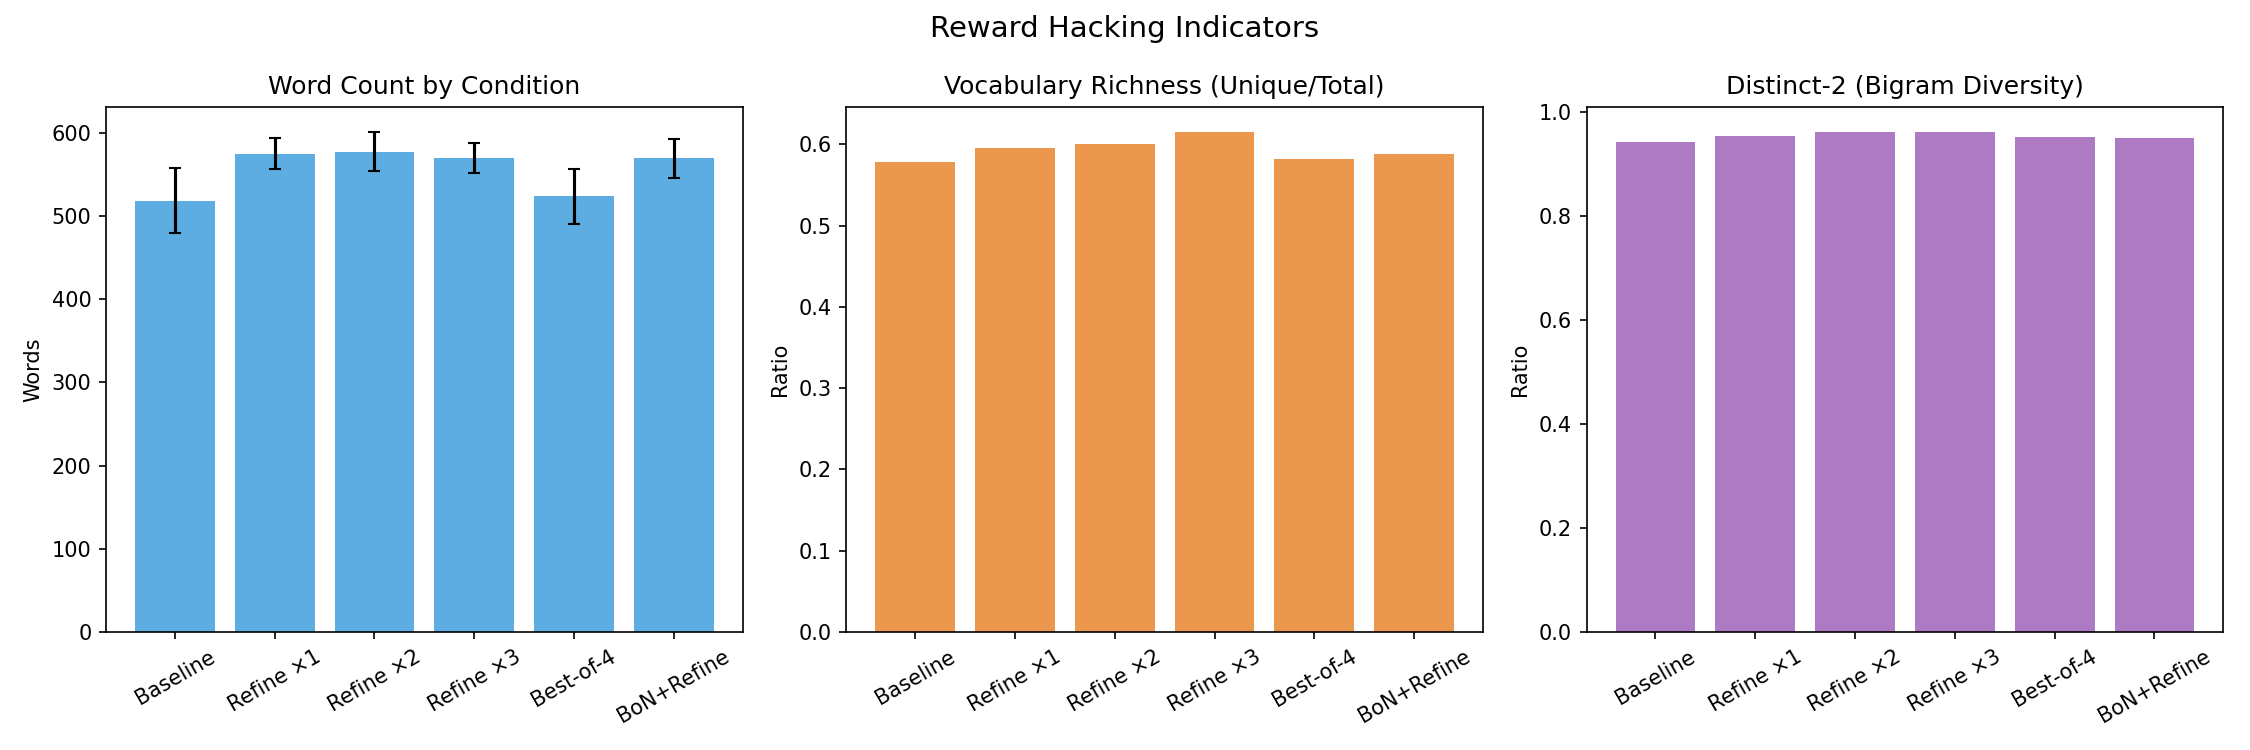
\includegraphics[width=0.75\linewidth]{figures/text_metrics.png}
\caption{Reward hacking indicators across conditions. Word count increases mildly (+11\%), while vocabulary richness and bigram diversity (Distinct-2) slightly improve, indicating no style collapse or superficial inflation.}
\label{fig:metrics}
\end{figure}

A key concern with self-critique is reward hacking---the model learning to exploit its own evaluation criteria through superficial changes~\citep{pan2024rewardhacking}.
\Figref{fig:metrics} and \tabref{tab:hacking} show that this does not occur in our setup.

\begin{table}[t]
\centering
\caption{Text-level metrics across conditions. Self-critique produces mild length increase and slightly improved lexical diversity.}
\label{tab:hacking}
\begin{tabular}{@{}lccc@{}}
\toprule
\textbf{Metric} & \textbf{Baseline} & \textbf{Refine $\times$1} & \textbf{Refine $\times$3} \\
\midrule
Word count & 518 $\pm$ 39 & 575 $\pm$ 19 & 570 $\pm$ 18 \\
Vocab richness (TTR) & 0.58 & 0.60 & 0.62 \\
Distinct-2 & 0.94 & 0.95 & 0.96 \\
\bottomrule
\end{tabular}
\end{table}

Word count increases by only 11\%, well below the 2.3$\times$ inflation reported by \citet{yuan2024selfrewarding}.
Vocabulary richness and n-gram diversity \emph{increase} slightly, contrary to the style collapse hypothesis.
This is partly attributable to our system prompt constraining story length to 400--600 words, but also suggests that self-critique pushes the model toward more varied language rather than repetitive elaboration.
